\documentclass{my_cv}
\usepackage{titlesec}
\usepackage{graphicx}
\usepackage{hyperref}
\begin{document}
	\name{Anuj Trehan}
	
	\begin{center}
		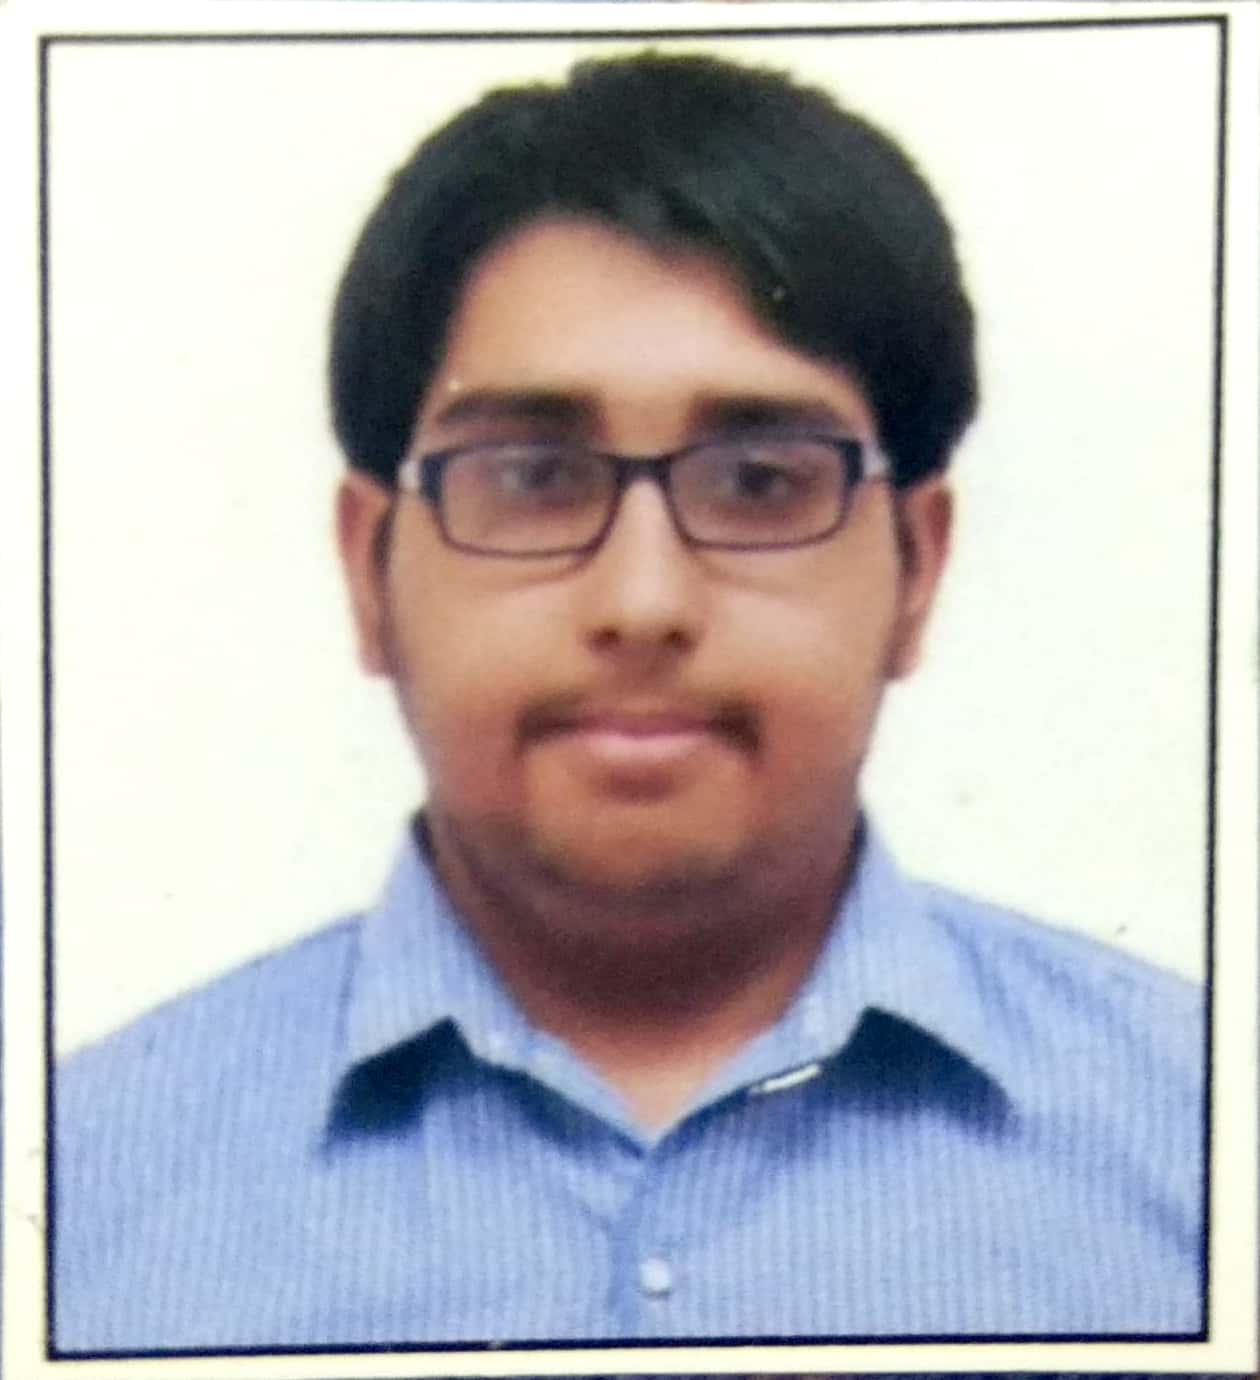
\includegraphics[width=3cm, height=3cm]{Anuj.jpg}\\
	\end{center}
	
	\contact{C-45 New Krishna Park,Vikas Puri}{New Delhi-18}{atrehan789@gmail.com}{+91 9999616069}
	
	\section{Career Objective}
	
	
	The main goal of my career is to help people using Artificial Intelligence and Internet as in my opinion if these two can be combined and used correctly we can create wonders.Also I believe in the power of education and have a vision to empower everyone with right type of education.
	
	\section{Education}
	
	\begin{tabular}{|l|l|l|l|l|}
		\hline
		Deg./Sem & Institute & University/Board & Passing year & Perc/CGPA \\
		\hline
		Semester 2 & B.V.C.O.E. & G.G.S.I.P.U. & 2018 & 9 \\
		\hline
		Semester 1 & B.V.C.O.E. & G.G.S.I.P.U. & 2017-18 & 9 \\
		\hline
		AISSCE & St. Cecilia\'s Public School & CBSE & 2017 & 92.4\%  \\
		\hline
		
		10$^{th}$ Board & St\. Cecilia\'s Public School & CBSE & 2015 & 9.4  \\
		\hline
	\end{tabular}
	\section{Projects}
	  \subsection{Music Generation with Deep Learning}
	  A LSTM network which is used for generating music note-by-note.\\
	  \href{ https://github.com/anuj2110/lstm-music-gen}{lstm-music-gen}
	  \subsection{Image Generation With Deep Learning}
	  Various autoencoders to generate images.\\
	  \href{https://github.com/anuj2110/keras}{Image Generation}
	  \subsection{Lane Detection With Computer Vision}
	  A program that can highlight lane lines on road in images and videos.\\
	  \href{https://github.com/anuj2110/LaneDetection}{Lane Detection}
	  \subsection{Painting With Deep Learning}
	  An algorithm which uses an image of painting to style a given image.\\
	  \href{https://github.com/anuj2110/neural-style-transfer
	  }{Neural Style Transfer}
	
    \section{Personal Details}
      
      
    \begin{tabular}{ll}
    	\textsc{Father's Name:} & Harish Trehan \\
    	\textsc{Mother's Name:}       & Bhawna Trehan \\
    	\textsc{Gender:}         & Male \\
    	\textsc{Date Of Birth:}         & 21 October 1998 \\
    	\textsc{Nationality:}   & Indian \\
    	\textsc{Marital Status:} & Single \\
    \end{tabular}
	

\end{document}
 